%----------------------------------------------------------------------------
\chapter{Computer vision}
\label{chap:perceptions}
%----------------------------------------------------------------------------

After collecting data from the sensors we choose we need to implement the right
algorithms to extract information from the sensor data. In this chapter I start
with explaining basics of computer vision and then move on to advanced
convolutional neural netowrks that will help our goal.

Computer Vision, often abbreviated as CV, is defined as a field of study that
seeks to develop techniques to help computers “see” and understand the content
of digital images such as photographs and videos.

The problem of computer vision appears simple because it is trivially solved by
people, even babies. Nevertheless, it largely remains an unsolved
problem based both on the limited understanding of biological vision and because
of the complexity of vision perception in a dynamic and nearly infinitely
varying physical world.

\section{Challenges in Computer Vision}
Image Classification is considered to be the most basic application of computer
vision. Rest of the other developments in computer vision are achieved by making
small enhancements on top of this. In real life, every time we, humans open our
eyes, we unconsciously classify and detect objects.

Since it is intuitive for us, we fail to appreciate the key challenges involved
when we try to design systems similar to our eye. Some challenges for computers are:

\begin{itemize}
    \item Variations in viewpoint
    \item Difference in illumination
    \item Hidden parts of images, occulsion
    \item Background Clutter
\end{itemize}

\section{Traditional approaches}

Various techniques, other than deep learning are available enhancing computer
vision. Though, they work well for simpler problems, but as the data become huge
and the task becomes complex, they are no substitute for deep CNNs. Let’s
briefly discuss two simple approaches.

\subsection{KNN (K-Nearest Neighbours)}

In the KNN algorithm each image is matched with all images in training data. The
top K with minimum distances are selected. The majority class of those top K is
predicted as output class of the image. Various distance metrics can be used
like L1 distance (sum of absolute distance), L2 distance (sum of squares), etc.
However KNN performs poorly - qute expectedly - they have a high error rate on
complex images, because all they do is compare pixel values among other images,
without any use of image patterns.

\subsection{Linear Classifiers}

They use a parametric approach where each pixel value is considered as a
parameter. It’s like a weighted sum of the pixel values with the dimension of
the weights matrix depending on the number of outcomes. Intuitively, we can
understand this in terms of a template. The weighted sum of pixels forms a
template image which is matched with every image. This will also face difficulty
in overcoming the challenges discussed in earlier as it is difficult to design a
single template for all the different cases.

\section{Convolutional Neural Networks}

Visual recognition tasks such as image classification, localization, and
detection are key components of Computer vision. However these are not possible
to achieve with traditional vision.

Recent developments in neural networks and deep learning approaches have greatly
advanced the performance of these state-of-the-art visual recognition systems.

Neural networks are the basis of deep learning methods. They are made up of
multiple layers, each layer containing multiple perceptrons. Layers can be
fully-connected or sparsely if possible, providing some performance benefits.
Each perceptron is an activation function whose input is the weighted output of
perceptrons from previous layers, and the function is usually a sigmoid
function. A neural networks first layer is the input layer and the last layer is
the output, which could be an array of perceptron where only one yields a high
output creating a classifier. Layer in-between are called hidden layers and it
is up to design and experimentation the determine what is the right
configuration of hidden layers.

\begin{figure}[!ht]
    \centering
    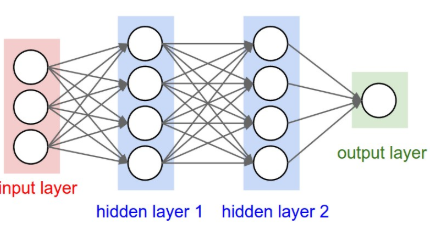
\includegraphics[width=80mm, keepaspectratio]{figures/nn.png}
    \caption{Neural network visualization. Image taken from CS231N Notes}
    \label{fig:convnet}
\end{figure}

Neural Networks (NN) are good at classifying different patterns recieved in the
input layers however they are not sufficient for even image classification,
because in one part the number of inputs is way to high. Consider a high
resolution image with $1000\times 1000\times 3$ pixels, then the NN has 3million input
parameters to process. This takes a long time and too much computational power.

Secondly the neural network architecture in itself is not a
general-enough solution (if you think about it, it is similar to a linear
classifier or a KNN).

Convolutional Neural Network (CNNs) however solve image classification and more.
A CNN is able to capture the spatial features in an image through the
application of relevant filters. The architecture performs a better fitting to
an image dataset due to the reduction in the number of parameters involved and
reusability of weights.


There is material on the internet in abundance about how convolutional neural
networks work, and I have read many of them, but the one I recommend most is the
Stanford course CS231N\footnote{ Stanford CV course CS231N
\url{https://cs231n.github.io/}}. 

The general architecture of CNN is similar to a cone, where the first layer is
the widest and each layer first convolves multiple filters (which in the
beginning of the CNN correspond to edges and corners) applying ReLU (rectifier,
non-linearity function) then it downsizes the input which is called the max
pooling. This repeated over and over in the end results in a small tensor
which can \emph{then} be fed to the fully-connected (FC) layers (i.e. a neural network)
which acts as the classifier.

Why is this the winner architecture? Because if you think about it the neural
network in the end only has to vote for the presence of the right features in roughly
the right image position, not for each pixel. A visualization of a
CNN's architecture can be seen in \autoref{fig:convnet}.

\begin{figure}[!ht]
    \centering
    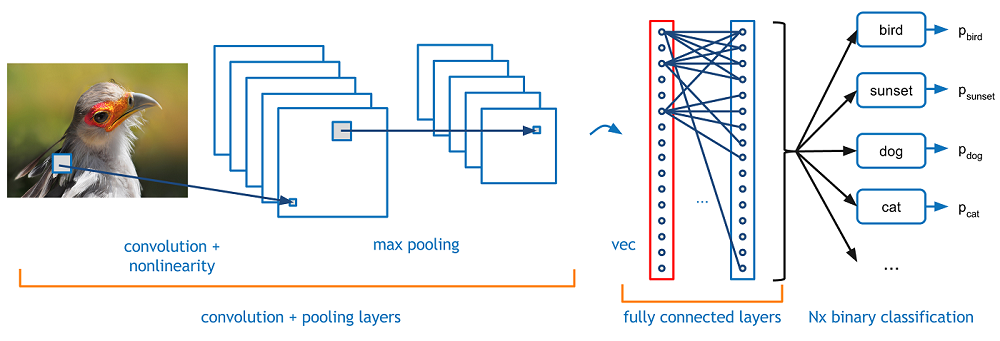
\includegraphics[width=150mm, keepaspectratio]{figures/convnet.png}
    \caption{Architecture of a CNN}
    \label{fig:convnet}
\end{figure}

\begin{figure}[!ht]
    \centering
    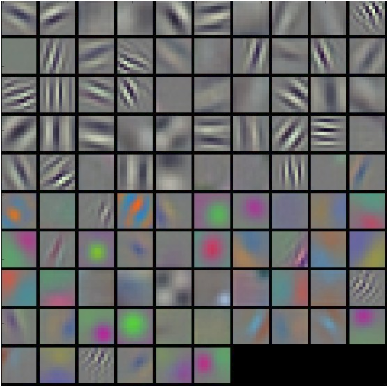
\includegraphics[width=60mm, keepaspectratio]{figures/filters.png}
    \caption{A visualization of the features learned in the first convnet layer in AlexNet~\cite{NIPS2012_4824}. AlexNet was a CNN which revolutionized the field of Deep Learning, and is built from conv layers, max-pooling layers and FC layers. Image taken from CS231N notes.}
    \label{fig:filters}
\end{figure}

There are various architectures that have emerged each incrementally improving on the previous ones:
LeNet~\cite{Lecun98gradient-basedlearning} - the work of Yann LeCun himself,
AlexNet~\cite{NIPS2012_4824}
VGGNet~\cite{DBLP:journals/corr/SimonyanZ14a}
GoogLeNet~\cite{DBLP:journals/corr/SzegedyLJSRAEVR14}
ResNet~\cite{DBLP:journals/corr/HeZRS15}

\subsection{Deep Learning}
Deep learning referes to the procedure of training neural networks and
convolutional neural networks to perform the task at hand accurately. During
deep learning first a dataset is created with training images coupled with
"ground truth" data that is the required prediction for each image. The neural
networks are then fed with the images in batches for a certain number of
iterations - epochs. The weights of the neural network and the filters are
adjusted with the loss function that comes from calculating the error of the
current prediction and the ground truth for each image. This error is then
"backpropagated" which is just another way of saying it is multiplied with the
derivative of each weight in the network and subtracted from it. For filters this means
"filtering filters", so only those filters will stay in the convnet which
resulted in a non-zero gradient in the neural network.

\section{Detection, Classification and Segmentation}
\subsection{Image Classification}

\subsection{Object Detection, Localization}
    (AlexNet, LeNet, VGG)
    R-CNN, Fast, Faster
    YOLO
\subsection{Segmentation}
Segmentation Networks
\subsection{Instance Segmentation}
Mask R-CNN - Detectron2
Yolact
Yolact++
\section{Tracking}
others
SORT
Deep Sort
\section{Bounding box detection and orientation}

\section{Key point detection}

\section{Voxelization}
PointNet
VoxelNet
\section{Lane and road detection}
Traditional way
Road detection
Driveable Road
Lane detection: sliding window, curve fit
\section{3D vision}
Camera model and Calibration
3D reconstruction
Stereo vision
Depth estimation
\section{Datasets}
Datasets - KITTI, MARS, COCO, Waymo, nuScenes









